\chapter{Implementação}
\label{chap:impl}

Neste capítulo discutiremos tópicos relacionados à implementação do sistema de diarização de locutor proposto. 

Na seção \ref{sec:tools} apresentamos as ferramentas principais utilizadas no desenvolvimento deste trabalho. Em seguida, na seção \ref{sec:preproc}, apresentamos o trabalho realizado para preparação e pré-processamento dos dados. Na seção \ref{sec:sysarch} discutimos a arquitetura do sistema desenvolvido, discussão esta que aprofundamos na seção \ref{sec:topology} através da demonstração da topologia da rede neural utilizada.

\section{Ferramentas}
\label{sec:tools}

Nesta seção apresentamos as principais ferramentas utilizadas durante a implementação deste trabalho. Definiremos suas principais características, assim como as funcionalidades das mesmas que foram utilizadas, e as motivações por trás de sua escolha.

Na seção \ref{subsec:dlib} apresentaremos a biblioteca dlib, utilizada para propósito de reconhecimento e demarcação facial no projeto. Em seguida, na seção \ref{subsec:tf} apresentaremos a biblioteca Tensorflow, utilizada por sua robusta implementação de rede neural. Na seção \ref{subsec:environ} apresentaremos o ambiente utilizado para treinamento do modelo, assim como seus recursos computacionais. Por fim, na seção \ref{subsec:otools}, mencionaremos brevemente as demais ferramentas utilizadas em caráter pontual no trabalho, e que, portanto, não receberam seções dedicadas.

\subsection{Dlib}
\label{subsec:dlib}
A Dlib\cite{dlib09} é uma biblioteca de código aberto desenvolvida em C++ e com interface em Python, com foco principal aplicação se encontra na área de processamento de imagens e reconhecimento facial. 

A biblioteca possui um reconhecedor facial frontal baseado em \textit{Histogram of Oriented Gradients} (HOG) capaz de detectar rostos frontais mesmo em imagens de baixa resolução. As características específicas deste reconhecedor estão discutidas na seção \ref{sec:faciallm}.

% FIXME: Colocar mais aprofundadamente na fundamentação teórica
% HOG é uma técnica de visão computacional na qual são calculados gradientes para cada pixel da imagem a partir de seus vizinhos de forma a identificar as fronteiras entre os objetos da figura. Os gradientes calculados são então utilizados para computar blocos descritores de 8x8 pixels com 9 canais. Esses blocos sofrem normalização local para compensar fatores como a iluminação do ambiente, e servem como entrada para uma Máquina de Vetores de Suporte, resultando em um reconhecedor de faces rápido e robusto. Uma explicação mais aprofundada sobre esta técnica pode ser obtida em \cite{dalalHistogramsOrientedGradients2005}.

\begin{figure}[ht]
    \centering
    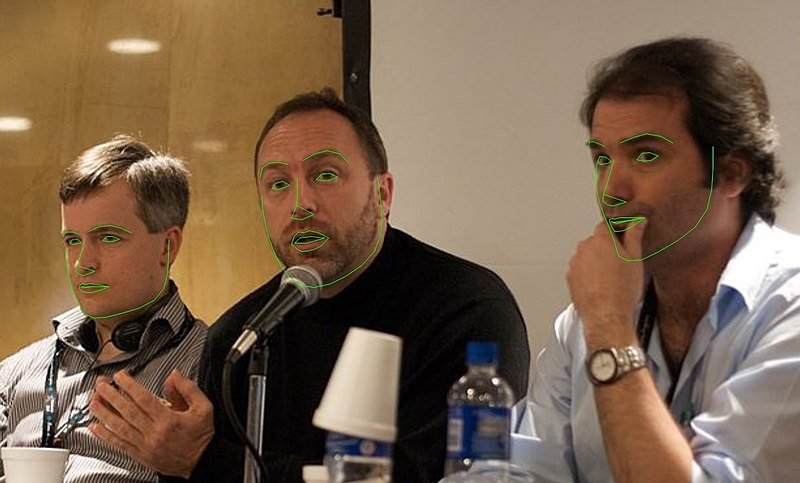
\includegraphics[width=0.7\textwidth]{dlib-face_landmark_detection.jpg}    
    \caption{Detecção de Marcadores Faciais pela biblioteca Dlib. Imagem publicada sob licença Creative Commons\cite{mtheilerDeteccaoMarcadoresFaciais2019}. }
    \label{fig:dlib-landmarking}
\end{figure}

Além disso, a biblioteca implementa um detector de marcadores faciais baseado em uma floresta de árvores de regressão, capaz de identificar (ou estimar, caso não estejam visíveis) as posições de um conjunto de pontos em um rosto, como mostra a figura \ref{fig:dlib-landmarking}. A biblioteca fornece também um modelo pré-treinado para este detector para identificação de 68 destes marcadores, sob licença que permite uso acadêmico. Esta funcionalidade foi chave para a escolha dessa biblioteca para a implementação do trabalho, visto que permitiu o treinamento do classificador utilizando um conjunto exponencialmente menor de dados, sem preocupações quanto a biases relacionados às características físicas do locutor.

\subsection{Tensorflow}
\label{subsec:tf}

Tensorflow\cite{tensorflow2015-whitepaper} é um framework de código aberto para aplicações de aprendizado de máquina. A biblioteca, construída pela Google, apresenta implementações robustas de diversos algoritmos da área, além de uma API que permite a declaração de uma rede neural em função de suas camadas. A biblioteca suporta, ainda, o uso de uma ou mais GPUs para treinamento da rede neural, através da biblioteca cuDNN. No trabalho, o Tensorflow foi utilizada para modelagem da rede neural, assim como o treinamento e posterior execução desta.

Sua escolha para o propósito do trabalho se deu devido à sua implementação de algoritmos chave para o desenvolvimento deste, tais como a rede neural convolucional tridimensional, discutida na seção \ref{sec:3dcnn}. Além disso, suas interfaces nas linguagens de programação C++ e Python, viculadas à facilidade de utilização da interface em Python da biblioteca, foram decisivas para a escolha desta para a realização do trabalho.

\subsection{Ambiente de Desenvolvimento}
\label{subsec:environ}

No desenvolvimento deste trabalho foi utilizada em caráter primário a linguagem de programação Python. Originalmente, o trabalho seria desenvolvido em C++ devido ao mais alto desempenho desta linguagem, porém a utilização de diversas bibliotecas com interface em Pythona ssim como sua facilidade de prototipagem levou à decisão de utiliza-la para a implementação final do projeto.

A IDE utilizada no desenvolvimento foi o Visual Studio Code, ferramenta de código aberto criada pela Microsoft, e o Jupyter Notebook\cite{Kluyver:2016aa}, por sua capacidade de subdividir e visualizar com facilidade o estado do programa em execução.

O treinamento da rede neural foi realizado em máquina com sistema operacional Windows, equipado com uma CPU Intel Core i7 de quarta geração, 12 GB de memória RAM e uma GPU Nvidia GTX 980 com 4 GB de VRAM.

\subsection{Outras Ferramentas}
\label{subsec:otools}

Nesta seção apresentamos as demais bibliotecas utilizadas no desenvolvimento do projeto. Em cada subseção descrevemos brevemente a biblioteca, definindo seu papel no projeto.

As bibliotecas se encontram ordenadas por sua função na pipeline do classificador, discutida de forma mais aprofundada na seção \ref{sec:sysarch}.

\subsubsection{OpenCV}

OpenCV\cite{opencv_library} é uma biblioteca de código aberto para aplicações de Visão Computacional. Ela foi utilizada para realizar a leitura quadro a quadro dos arquivos de vídeo a serem processados pelo sistema, e para codificar em video a saída do classificador.

\subsubsection{Matplotlib}

A Matplotlib\cite{Hunter:2007} é uma biblioteca para produção de gráficos e imagens em Python. Ela foi utilizada para produzir as imagens intermediárias, através do desenho de polígonos a partir dos vértices produzidos pelo processo de marcação facial.

\subsubsection{Pandas}

Pandas\cite{mckinney-proc-scipy-2010} é uma biblioteca de processamento de dados em Python. Ela foi utilizada no préprocessamento dos dados com a finalidade de manipular os arquivos csv produzidos pelo processo de diarização manual dos videos do dataset de depoimentos.

\section{Preparação dos Dados}
\label{sec:preproc}

Originalmente, foi fornecido pela Defensoria Pública do Estado do Rio de Janeiro um dataset contendo cerca de 5 horas de vídeo, divididas em 30 vídeos de depoimentos, cada um referente às declarações de um ou mais depoentes. Os videos fornecidos apresenta resolução de $320\times240$ pixels, a uma taxa de 30 quadros por segundo. O conjunto de dados não apresentava nenhuma anotação quanto à fala do depoente, portanto nossa primeira etapa foi constituída pela diarização manual de alguns dos videos fornecidos.

A primeira etapa foi constituída pela segmentação dos videos em fragmentos de 15 quadros, ou meio segundo. A motivação para a segmentação do video de entrada em trechos deste comprimento foi a estipulação de que o tempo necessário para a fala da primeira sílaba em uma frase por uma pessoa normal, no português do Brasil, é de 252 milisegundos\cite{barbosaSyllabletimingBrazilianPortuguese2000}, o que constitui cerca de metade desse tempo. Sendo assim, julgamos que seria possível detectar mesmo falas curtas considerando este o tamanho da janela.

Estes trechos foram validados para determinar se a face do depoente poderia ser reconhecida, com finalidade de descartar fragmentos nos quais este não olhava em direção à câmera. Posteriormente, cada trecho foi classificado quanto à ocorrência de fala pelo depoente, produzindo uma tabela que associava o identificador de cada arquivo à classe correspondente ao mesmo.

Feita a diarização, os videos foram separados em conjuntos de teste e treinamento, tais que vídeos diferentes seriam utilizados para cada fase do treinamento da rede. Essa separação foi feita pois, como os fragmentos possuem relação temporal entre si, seria possível que o treinamento da rede neural utilizando segmentos imediatamente posteriores ao fragmento de teste pudesse inflar o desempenho da mesma nas predições realizadas sobre este.

Por fim, as diarizações produzidas manualmente foram utilizadas para organizar os fragmentos em uma estrutura de diretórios, tal que a primeiramente estivessem separados por conjunto de teste ou treinamento, depois por classe, e por fim por vídeo de origem. Essa estrutura foi construída tal que as informações relevantes ao gerador de amostras da rede neural pudessem ser obtidas todas a partir do caminho para o mesmo.

Para a execução de todas essas tarefas foram desenvolvidos scripts em Python e Bash, capazes de segmentar o dataset e de validar, mover, e organizar os fragmentos que o compõem. O código referente a estes pode ser encontrado no apêndice \ref{apdx:src}.

\section{Arquitetura do Sistema}
\label{sec:sysarch}

Foram desenvolvidos dois conjuntos scripts distintos para este trabalho; um sistema para treinamento da rede neural convolucional, e outro para a diarização de locutor em um vídeo com as características definidas anteriormente. Sendo assim, discutiremos a arquitetura utilizada para treinamento do modelo na seção \ref{subsec:train}, e a utilizada no processamento de uma mídia de entrada na seção \ref{subsec:application}.

\subsection{Treinamento}
\label{subsec:train}

A arquitetura do sistema de treinamento consiste em um gerador de dados e um modelo de rede neural convolucional a ser treinado.

% \input{figures/arch-train}

A função primária do gerador de dados é carregar dinâmicamente os vídeos a serem alimentados ao modelo em cada etapa de seu treinamento. Para isto, ele é inicializado com uma lista dos arquivos a serem carregados, assim como uma série de parâmetros que definem aspectos de sua operação, tais como o tamanho da batelada ou o pré-processamento a ser aplicado aos quadros.

\begin{figure}[ht]
    \centering
    \includesvg[width=0.85\textwidth]{loader_rgb.svg}
    \includesvg[width=0.85\textwidth]{loader_gray.svg}
    \includesvg[width=0.85\textwidth]{loader_lm.svg}
    \caption{Os três modos de operação do gerador de dados.}
    \label{fig:train_metrics_evo}
\end{figure}

O gerador de dados possui 3 modos distintos de operação. Estes são:
\begin{itemize}
    \item RGB: Nesse modo, o quadro é retornado como uma imagem em padrão RGB, ou seja, com suas cores representadas por suas componentes vermelha, verde, e azul, nesta ordem.
    \item Grayscale: Nesse modo, o quadro é retornado convertido para escala de cinza, segundo a função $Y = 0.299 R + 0.587 G + 0.114 B$.
    \item Landmarks: Nesse modo, é gerada uma imagem em preto e branco, rasterizada a partir dos pontos identificados pela detecção de marcadores faciais em cada quadro carregado. Este foi o modo utilizado na implementação final do trabalho.
\end{itemize}
O gerador é capaz, ainda, de manter um \textit{cache} atualizado com os cálculos realizados no carregamento dos quadros, a fim de possibilitar treinamento mais rápido do modelo em épocas consecutivas.

Em nossa implementação final, utilizamos o modo de \textit{landmarks}. Esse modo consiste em três operações consecutivas; primeiramente, o segmento de video é carregado do disco quadro a quadro. Depois, estes quadros sofrem reconhecimento facial e, em seguida, as faces detectadas passam pelo detector de marcadores faciais, que retorna o conjunto de 68 pontos correspondentes aos marcadores detectados. Estes pontos são, então, utilizados para o desenho de polígonos sobre um canvas branco de mesmo tamanho da imagem original, na etapa que chamamos de rasterização. Essa etapa garante a preservação das relações entre os marcadores faciais. Por fim, a imagem rasterizada é recortada segundo o retângulo delimitado pelo reconhecedor facial e alinhada horizontalmente.

Em seguida, configuramos o modelo da rede neural. Os detalhes e decisões referentes à configuração deste podem ser encontradas na seção \ref{sec:topology}. O treinamento é então realizado em um loop. Como critérios de parada, utilizamos um limite de 100 épocas no treinamento. Como medida de prevenção ao \textit{overfitting} na rede neural, paramos o treinamento quando o valor da função custo no conjunto de validação não for reduzido em um período de três épocas.

\begin{equation} \label{eq:categorical_crossentropy}
    L(y,\hat{y})=-\sum\limits_{j=0}^M\sum\limits_{i=0}^N(y_{ij}*log(\hat{y}_{ij}))
\end{equation}

Como função de custo, dado que estamos lidando com um problema de classificação, utilizamos a função de entropia categórica cruzada, ou \textit{custo softmax} (equação \ref{eq:categorical_crossentropy}). Nessa equação, $\hat{y}$ é o vetor das probabilidades das categorias, e $y$ é a categoria real, codificada \textit{one-hot}.

Em cada época, o modelo chama o gerador de dados de treinamento, que lhe retorna uma batelada composta por um número fixo de amostras. Cada uma dessas amostras é, como discutido anteriormente, um segmento de 15 quadros consecutivos, extraído de um vídeo e pré-processado pelo gerador. Ao esgotarem as amostras de teste, o modelo chama, então, o gerador de dados de validação, realizando predições sem retropropagação sobre as entradas retornadas, e calculando o valor da função custo para os resultados. Por fim, ao se esgotarem também essas amostras, dá-se o final de uma época de treinamento, e os geradores tem suas listas de arquivos embaralhadas de forma a garantir aleatoriedade na ordem da próxima época.

\begin{figure}[ht]
    \centering
    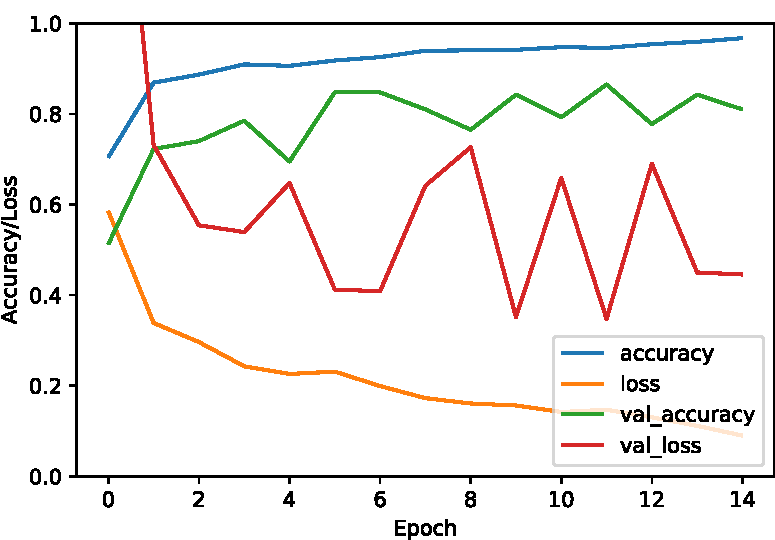
\includegraphics[width=0.5\textwidth]{training_metrics_evolution.pdf}
    \caption{Evolução das métricas do treinamento ao longo do tempo. A métrica val\_loss, valor da função custo sobre os resultados do conjunto de validação, foi critério de parada do treinamento.}
    \label{fig:train_metrics_evo}
\end{figure}

O processo de trinamento do modelo levou 15 épocas em nosso treinamento inicial, como mostra a figura \ref{fig:train_metrics_evo}. Ao fim do processo, os pesos com menor custo no conjunto de validação foram restaurados.

\subsection{Aplicação}
\label{subsec:application}

% \input{figures/arch-run}

% TODO: Escrever sobre a arquitetura do sistema

\section{Topologia da Rede Neural}
\label{sec:topology}

% TODO: Escrever sobre a topologia da rede neural